% =============================================================================
% Section 2.1: Targeted Customers
% =============================================================================

\section{Targeted Customers}
\label{sec:targeted-customers}

NexaLearn is architected as a backend \textit{platform} rather than a turnkey consumer-facing application. Its modular monolith design, OpenAPI-documented REST surface, Docker Compose deployment, and explicit bounded contexts make it most valuable to organisations that employ software engineers and require deep customisation, data sovereignty, or integration with existing identity, billing, and content systems. Three customer segments---primary, secondary, and tertiary---emerge from this positioning, each with distinct pain points that NexaLearn's architecture addresses directly.

\subsection{Primary Segment: EdTech Startups and Independent Developers}
\label{subsec:primary-edtech}

The \textbf{primary target segment} comprises edtech startups, independent software developers, and small product teams building online learning marketplaces, niche certification platforms, or vertical training products (e.g., medical continuing education, creative skills, language tutoring). These customers typically possess TypeScript or Node.js competency but lack the calendar months required to implement production-grade payment sagas, Mux-integrated video lifecycles, transactional outbox event processing, and AI pipeline orchestration from first principles.

\textbf{Pain points.} Generic NestJS boilerplates provide authentication scaffolding but omit enrollment state machines, Stripe webhook idempotency, and instructor analytics. Stitching together Stripe, Mux, SendGrid, and OpenAI APIs without a unified domain model produces fragile glue code that fails under duplicate webhook delivery or concurrent course edits. Venture-backed startups face investor scrutiny on time-to-market; bootstrapped founders face direct opportunity cost for every month spent reinventing outbox patterns instead of differentiating on curriculum or user experience.

\textbf{How NexaLearn benefits this segment.} NexaLearn delivers a \textit{reference implementation} with sixteen bounded contexts, 150+ documented endpoints, Testcontainers integration tests, and architecture documentation sufficient to fork and customise. Teams can deploy via Docker Compose on day one, replace branding and frontend independently, extend the Courses or Assessment contexts for domain-specific rules, and inherit reliability patterns (idempotency keys, optimistic locking, HMAC callbacks) without research overhead. The open-source core eliminates licensing fees during MVP validation; enterprise support becomes relevant only when SLAs, security reviews, or dedicated migration assistance are required at scale.

\textbf{Representative use cases} include a regional coding bootcamp launching a proprietary alumni learning portal, a startup white-labelling course delivery for influencer creators, and an agency building custom LMS backends for multiple clients from a shared NexaLearn fork.

\begin{figure}[H]
  \centering
  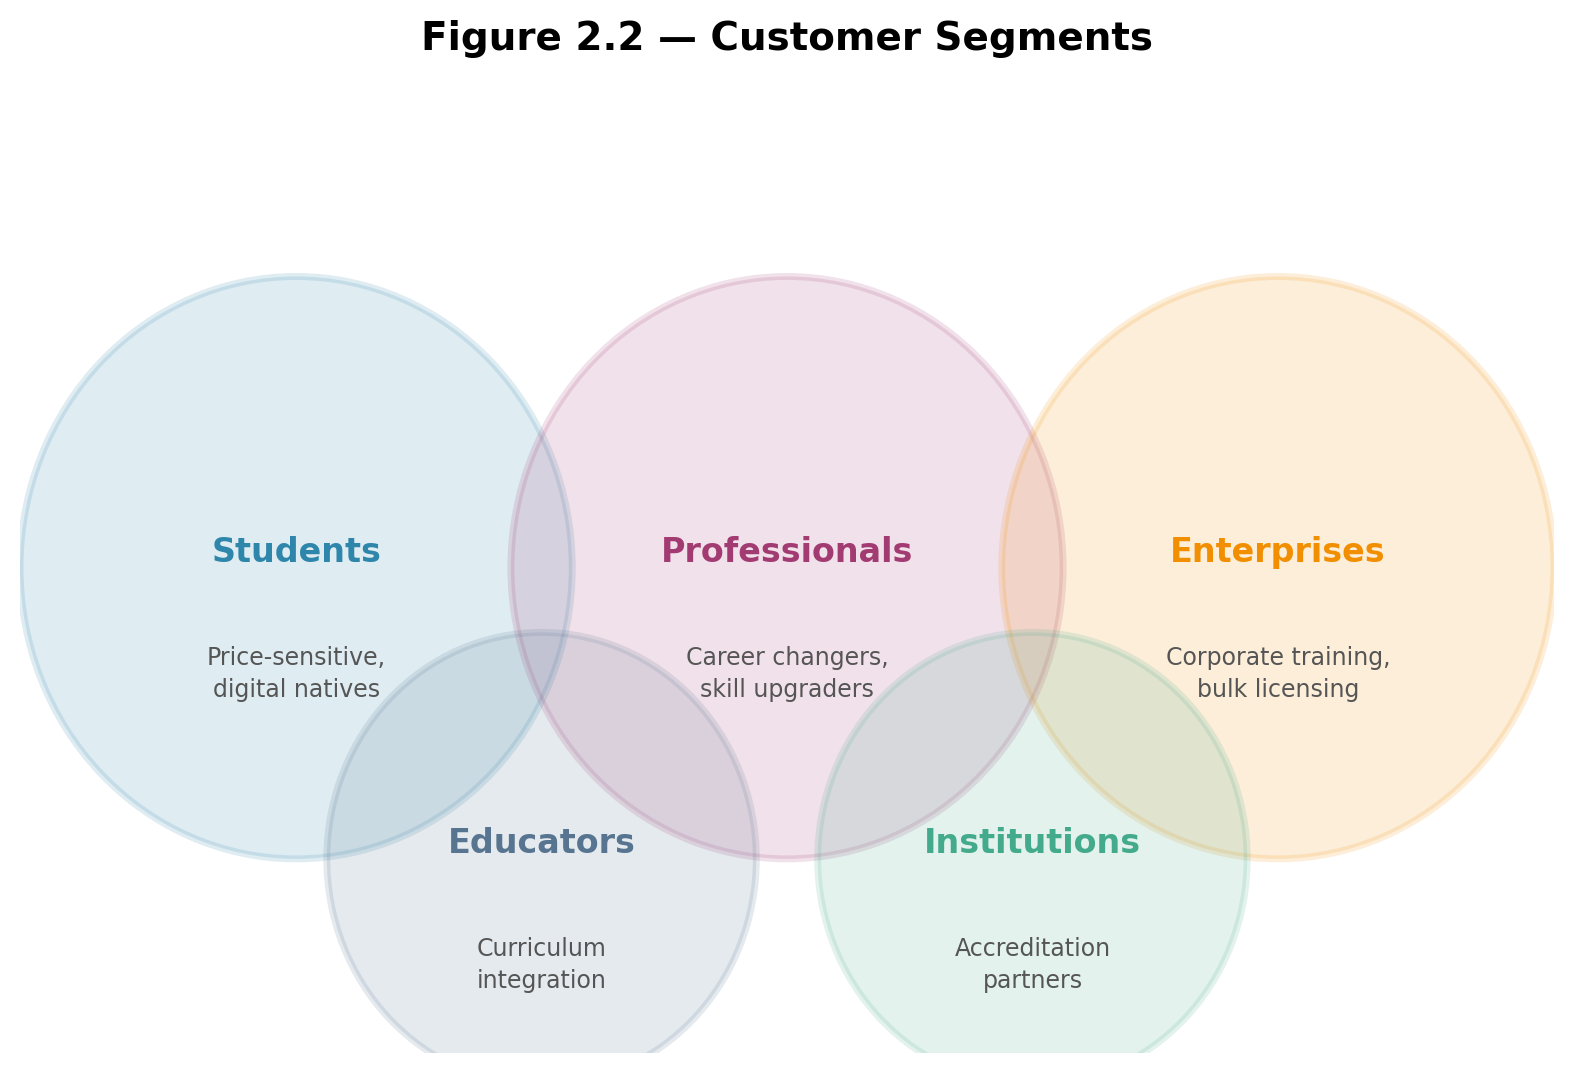
\includegraphics[width=0.88\textwidth]{images/customer_segments.png}
  \caption{NexaLearn Target Customer Segments and Value Proposition Alignment}
  \label{fig:customer-segments}
\end{figure}

Figure~\ref{fig:customer-segments} illustrates how NexaLearn's architectural strengths---open source, DDD modularity, AI pipeline integration, Stripe/Mux readiness---map most directly to developer-led edtech teams while remaining applicable to institutional and corporate buyers with internal engineering capacity.

\subsection{Secondary Segment: Universities and Educational Institutions}
\label{subsec:secondary-universities}

The \textbf{secondary segment} includes universities, faculties, and continuing-education departments seeking a \textbf{self-hosted} learning management backend under institutional data-governance policies. Public universities in Egypt and the broader MENA region increasingly require on-premise or sovereign-cloud deployment where student records, payment metadata, and proctored assessment data must not reside on unreviewed third-party SaaS infrastructure subject to foreign jurisdiction.

\textbf{Pain points.} Legacy Moodle deployments satisfy self-hosting requirements but burden IT departments with PHP plugin maintenance, inconsistent security patching, and limited TypeScript talent pools among student developers contributing to customisations. Commercial platforms such as Coursera for Campus offer polished experiences but constrain integration with existing Student Information Systems (SIS), restrict modifications to enrollment logic, and impose per-seat licensing that scales expensively across tens of thousands of registered students.

\textbf{How NexaLearn benefits this segment.} NexaLearn runs entirely on institution-controlled PostgreSQL and Redis instances, exposes REST APIs for SIS integration (enrollment sync, grade export), and supports RBAC roles aligned with academic hierarchies (student, instructor, department admin). The transactional audit module assists compliance officers reviewing administrative actions. AI-assisted quiz generation augments faculty workflows without mandating a specific frontend---faculties may build localised Arabic/English clients atop the API. Institutions with Computer Science departments may further extend NexaLearn as a living capstone platform, as demonstrated by this graduation project.

\textbf{Adoption pathway.} Pilot deployment for a single department (e.g., Computer Engineering online electives), evaluation against Moodle on maintainability and security criteria, and phased rollout with enterprise support covering migration tooling and SLA-backed incident response.

\subsection{Tertiary Segment: Corporate Training and L\&D Departments}
\label{subsec:tertiary-corporate}

The \textbf{tertiary segment} comprises mid-to-large enterprises operating internal \textbf{white-label} training programmes: employee onboarding, compliance certification (OSHA, ISO, financial regulations), sales enablement, and leadership development. These buyers prioritise SSO integration (SAML/OIDC), branded learner experiences, completion tracking for HR analytics, and cost predictability over marketplace discovery features irrelevant to internal audiences.

\textbf{Pain points.} Enterprise LMS suites (Cornerstone, SAP SuccessFactors) involve multi-year contracts, lengthy implementation cycles, and limited API access for custom mobile apps. Lightweight SaaS tools (Teachable, Thinkific) target creators rather than IT departments and lack SSO, audit trails, and horizontal scaling patterns for workforces numbering tens of thousands. Building in-house from scratch duplicates NexaLearn's sixteen-context scope unless engineering teams exceed twenty backend developers.

\textbf{How NexaLearn benefits this segment.} NexaLearn provides white-label readiness: self-hosted deployment behind corporate VPN or private cloud, custom domain and email templates via Notifications context, instructor analytics aggregated for L\&D managers without exposing individual performance to unauthorised managers (privacy-preserving query services described in Chapter~1), and Streak/Progress modules supporting compliance deadlines. The open-core model allows enterprises to audit source code during security review---a requirement absent from closed SaaS alternatives. Enterprise support at \$5,000/year per deployment instance is orders of magnitude below enterprise LMS licensing for comparable customisation freedom.

\subsection{Segment Prioritisation and Go-to-Market Implications}
\label{subsec:segment-prioritisation}

Table~\ref{tab:segment-summary} summarises segment prioritisation for commercialisation. The primary edtech developer segment drives open-source adoption metrics (stars, forks, community contributions) that reduce customer acquisition cost for enterprise support sales to secondary and tertiary buyers.

\begin{table}[H]
  \centering
  \caption{Customer Segment Summary and NexaLearn Fit}
  \label{tab:segment-summary}
  \small
  \begin{tabular}{@{}p{2.4cm} p{2.2cm} p{3.5cm} p{4.8cm}@{}}
    \toprule
    \textbf{Segment} & \textbf{Priority} & \textbf{Decision Maker} & \textbf{Key NexaLearn Advantage} \\
    \midrule
    EdTech startups \& indie developers &
    Primary &
    CTO / lead developer &
    Full source access; DDD reference; fast Docker deploy \\
    \addlinespace
    Universities \& institutions &
    Secondary &
    IT director / dean &
    Self-hosted; audit trail; SIS API integration \\
    \addlinespace
    Corporate L\&D &
    Tertiary &
    HR IT / L\&D manager &
    White-label; SSO-ready; compliance analytics \\
    \bottomrule
  \end{tabular}
\end{table}

In summary, NexaLearn's architecture is optimised for technically sophisticated buyers who value \textit{control, clarity, and extensibility} over turnkey drag-and-drop simplicity---a deliberate trade-off that aligns with the platform's graduation project origins and open-source commercialisation strategy developed in Section~\ref{sec:business-case}.
